\documentclass[a4paper]{article}

\usepackage{bnaic}
\usepackage{hyperref}
\usepackage[all]{hypcap}
\usepackage{graphicx}
\usepackage{float}
\usepackage{subcaption}
\usepackage{algorithm}
\usepackage{algpseudocode}

\title{Learning to play Hare and Hounds using Q-learning}
\author{Xeryus Stokkel \and Siegrid Lenting \and Ren\'e Mellema}

\begin{document}

\maketitle

\section{Introduction}
Hare and Hounds is a simple game with two players who alternate turns. One
player plays as the hare while the other plays as three hounds. The hounds
player gets to move first. The goal of the
hare is to escape the hounds while the goal of the hounds is to capture the
hare. The hare is captured when it cannot move on its turn. The hare has escaped
when it reaches the left side of the board. The board of the game is shown in
\autoref{fig:board}. The hounds also lose when they are considered stalling,
in most versions of the game this means that the hounds made the same
(vertical) move ten times in a row. The player who controls the hounds is only
allowed to move one hound per turn to adjacent squares that are to the right,
either horizontally or diagonally, or to move vertically. The hare can move in
any direction to an adjacent square. A square can only be occupied by one piece
at a time. While this game seems to be very simple it actually has quite deep
strategy \cite{gardner1961second}. 

The game is also known as The Soldier's game, Game of Dwarfs, French
Military Game or any other regional equivalent. Not all of these variants
use the same shaped board but we will focus on the board configuration
shown in \autoref{fig:board}. Other variations include longer or circular
boards.  Some variants of the game also use different rules. Our variant
uses a slightly altered set of rules from above. Instead of the hounds
loosing after stalling for ten turns in a row, our game has a maximum
length of 50 turns per player.  When this turn limit is reached the game is
considered a draw and neither player wins.  It is known that when using the
rules described above that the game is biased towards the
hounds \cite{gardner1961second}. Therefore, we expect the hounds to win all
games when  both players are fully trained. 

In this paper we will describe a method of learning to play the game of Hare
and Hounds using reinforcement learning. The methodology is explained in
\autoref{sec:method}, we discuss the results of training in
\autoref{sec:results} while final remarks are made in \autoref{sec:discussion}.

\begin{figure}[h]
    \centering
    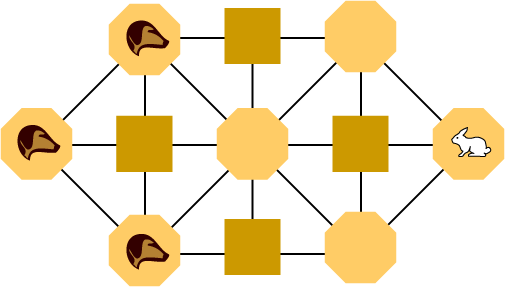
\includegraphics[width=.75\textwidth]{Hare_and_Hounds_board.png}
    \caption{The game board that Hare and Hounds is played on. The hare player
        starts on the right while the hounds player starts on the left.}
    \label{fig:board}
\end{figure}


\section{Method}\label{sec:method}
To learn how to play Hare and Hounds we will use Q-learning\cite{watkins1992q}.
Each player will be represented by a different Q-table. This means that the
actions of the hare are separate from those of the three hounds combined. We
did not opt for using a separate Q-table for each hound because the hounds are
suppose to be working together as they are the pieces of a single player.

To select the most appropriate action in each state we use the softmax
function. This means that during training we can move from exploration to
exploitation easily by adding a temperature parameter. When the temperature
is infinite then pure exploration is used while it would ensure pure
exploitation when its value is very small. The action selection function then
looks as follows
\[ P(a|s) = \frac{\exp[Q(s,a)/T]}{\sum_{b \in A} \exp[Q(s, b)/T]} \]
Where $P(a|s)$ is the probability that an action is selected in any state, $A$
is the set of available actions in a state, $Q(s,a)$ is the value from the
Q-table for a state-action pair and $T$ is the temperature parameter. During
training we linearly decrease the temperature by a single degree after every
game, the final temperature in the last game is one degree.

\section{Results}\label{sec:results}
Since the hounds will always win with optimal play from both sides, we can
use the percentage of wins from the hounds as a measure of performance. If
the hound win the majority of the games, then we can assume that the system is
fully trained. Therefore we decided to use this as a measure of performance. 

Graphs with the percentage of wins for the hounds for different
configurations can be found in \autoref{fig:dat}. Not all lines are visible
in \autoref{fig:r10000}, \autoref{fig:r100000}, and \autoref{fig:r5000000},
since the performance is so similar for different values of $\gamma$ that
they all lay on the same line and are therefore masked beneath eachother.

\begin{figure}[bt]
    \centering
    \begin{subfigure}{0.49\textwidth}
        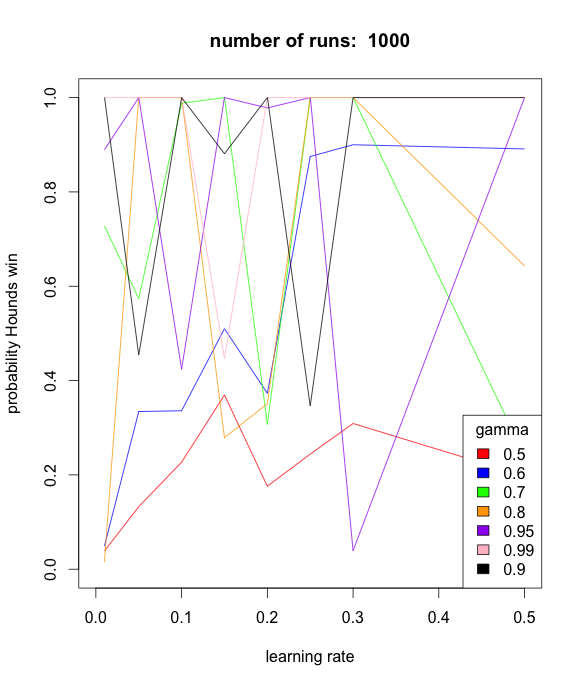
\includegraphics[width=\textwidth]{r1000}
        \caption{The percentage of wins for the hounds for different values
            of $\eta$ and $\gamma$ for 1000 runs}
        \label{fig:r1000}
    \end{subfigure}
    ~
    \begin{subfigure}{0.49\textwidth}
        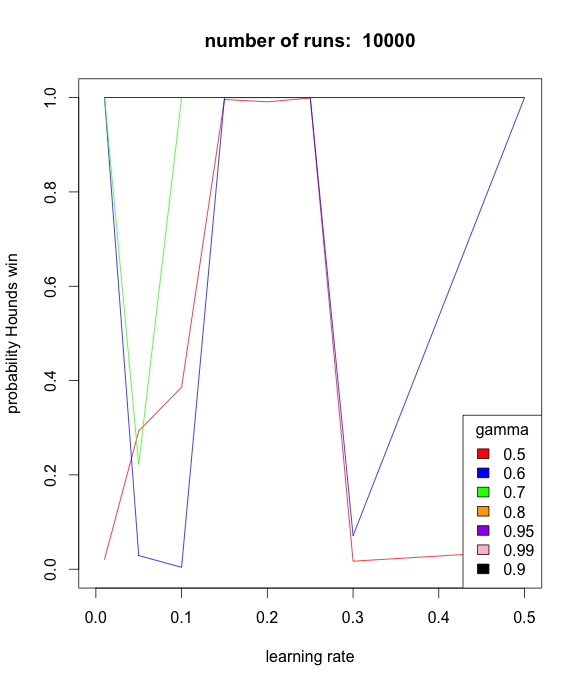
\includegraphics[width=\textwidth]{r10000}
        \caption{The percentage of wins for the hounds for different values
            of $\eta$ and $\gamma$ for 10000 runs}
        \label{fig:r10000}
    \end{subfigure}
    
    \begin{subfigure}{0.49\textwidth}
        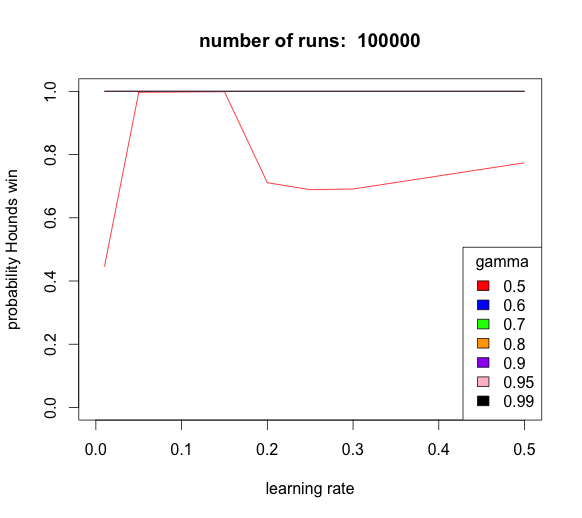
\includegraphics[width=\textwidth]{r100000}
        \caption{The percentage of wins for the hounds for different values
            of $\eta$ and $\gamma$ for 100000 runs}
        \label{fig:r100000}
    \end{subfigure}
    ~
    \begin{subfigure}{0.49\textwidth}
        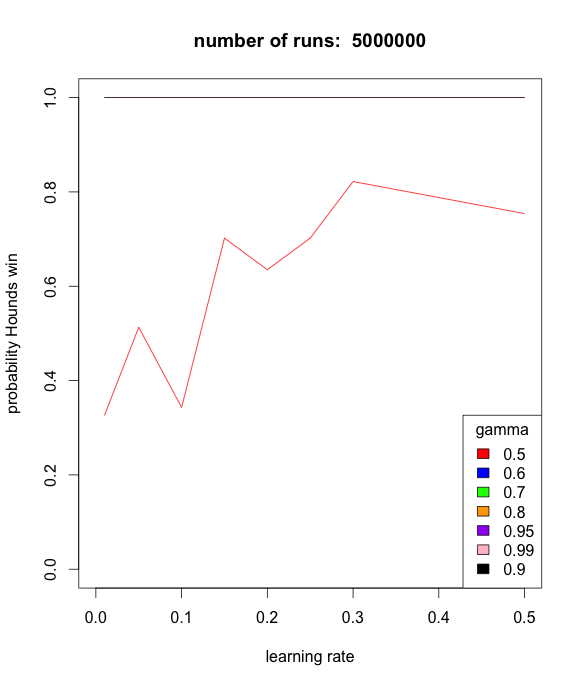
\includegraphics[width=\textwidth]{r5000000}
        \caption{The percentage of wins for the hounds for different values
            of $\eta$ and $\gamma$ for 5000000 runs}
        \label{fig:r5000000}
    \end{subfigure}
    \caption{The percentage of hounds wins for several configurations}
    \label{fig:dat}
\end{figure}

In the graphs we can see that after about 1000 training runs, for values of
$\gamma$ higher than $0.8$ and all values of $\eta$, the hounds always win.
From 10000 training runs and higher, this even goes for values of $\gamma$
of $0.6$ and higher. Here we can clearly see the effect of the discount
factor, if we have a lower discount factor, and therefore take a shorter
period of time into account, we have to train the system for longer than
when we focus more on the long run and therefore include more games.

What we can also see from \autoref{fig:r100000} and \autoref{fig:r5000000}
is that there is no difference in performance for all values of $\gamma$
higher than $0.6$ for this training time. That means that after 100000
training runs, one can stop training the system. For higher values of
$\gamma$, the system is already trained in 10000 training steps
(\autoref{fig:r10000})

We can also see that the value of $\eta$ does not have a large influence on
the eventual performance. This is not that unexpected, since the learning
rate is lowered over time, so for all values of $\eta$ it tends to 0 in
update proportional to the number of runs used for training and the
starting value of $\eta$. This means that after a few runs all values of
$\eta$ become similar.

To further see the influence of the paramters on the performance, we
constructed a linear model that can predict the performance based on the
parameters given. This model gives us similar results as we could see from
the graphs, with a high significance for the discount factor ($p < 1 \times
10 ^ {-11}$) and the number of runs ($p < 1 \times 10 ^ {-6}$), while the
value for the learning rate is not significant ($p = 0.281$). From this we
can confirm our suspicion that the value of the learning rate does not have a
great influence over the eventual performance.



\section{Discussion}\label{sec:discussion}
We can see that after enough training the hounds will always win for most of
parameter settings. \autoref{fig:r5000000} shows a horizontal line at 1.0 for
all parameters except when $\gamma = 0.5$. This means that the hounds player
always wins for each configuration where $\gamma \geq 0.6$. We can thus say
that these settings are optimal for the hounds player.

From \autoref{fig:dat} we can see that we need about 100 000 games for training
to converge. In \autoref{fig:r10000} we can see that 10 000 games are not enough
since some combinations of the different parameter configurations are not fully
horizontal yet, but that most of the configurations do end up in a state where
hounds always wins. The difference between 100 000 and 5 000 000 games is not
very large, we can even say that 5 000 000 games is slightly worse for the
hounds player but better for the hare player since some points are more
beneficial to the hare player. However this is not a very large difference and
thus we can conclude that it is not worth the extra training time.

Although the game does not have a very large state space because the board is
so small, it might still take up a large amount of memory to store it. We
decreased the size of the state space by not considering the hounds to be
unique. If the position of two hounds is swapped then the state remains the
same. If we did consider the hounds to be unique then the state would also
change when we swap the position of two hounds. Another way to decrease the
size of the state space is by exploiting the symmetry of the board. The board
is symmetrical horizontally so this means that we could consider states to be
equal when they are horizontally flipped versions of each other. Removing these
flipped versions would mean that the state space is also decreased. This might
also improve learning since there are far fewer states to learn in this case.

Another option to reduce storage complexity is to use one single table for both
players. In this case the hare player would select an action that would lead
to the outcome with the lowest reward, i.e. the largest negative value. This
should not lead to any problems with overlapping actions since the sets of
actions are disjoint. Our implementation models the possible actions of the
hounds player as moving a piece from one place to another while the set of
possible actions of the hare player is moving to a square. The difference
may be subtle but it means that one player could not possibly accidentally
pick the action of another player, nor can they update each other's Q-values.

Although we only used softmax to select the action that players should perform
we could also have opted for $\varepsilon$-greedy where the option to take a
random action is picked with probability $\varepsilon$, this would be the
proportion we want to explore. On the other hand the proportion of exploitation
is $1-\varepsilon$, in that case we pick the best known action. It could be
interesting to see the effect of using the softmax vs. the $\varepsilon$-greedy
method would be.

It seems that using reinforcement learning to learn to play the game Hound and
Hare works well. Using Q-learning gives us the results we would expect in
a decent about of training epochs. There are still interesting things that
could be done using this technique. In our study, we only compared the
performance of the hounds against a hare which was trained with the same
parameters. An interesting thing to test would be to compare a set of
hounds with different training parameters from the hare, so both players
might have had different discount factors during training, leading to
different kinds of behaviors.

Another interesting line of research would be to compare the learned policy
from Q-learning with the policies found in combinatorial game theory
\cite{gardner1961second, siegel2005coping}. If these policies are the same,
then Q-learning does indeed learn the optimal policy, but if they are
different the reinforcement learning method might not have searched through
the state space sufficiently enough. On the other hand, Q-learning might
also find better policy than the combinatorial game theorists have found,
sparking new research in that area.


\bibliographystyle{plain}
\bibliography{literature}

\end{document}
